%\documentclass[12pt,a4paper]{report}
\documentclass[12pt,a4paper,oneside,onecolumn,openright]{book}
% set the document language
\usepackage[italian]{babel}
% set the encoding used by your editor here (default is utf8)
\usepackage[utf8]{inputenc}

% math packages
\usepackage{amsmath}
\usepackage{amssymb}
% page margins settings
\usepackage[inner=3cm,outer=2.5cm,top=3cm,bottom=2.5cm]{geometry}
%\usepackage{indentfirst}


% other packages
\usepackage{array}
\usepackage{subfigure}
\usepackage{graphicx}
\usepackage{verbatim}
\usepackage{listings}
\usepackage{url}
\usepackage[hidelinks]{hyperref}
\usepackage{wrapfig,lipsum,booktabs}
\usepackage[sorting=none]{biblatex} %Imports biblatex package

\usepackage{pgfplots}
\pgfplotsset{width=10cm,compat=1.9}

% We will externalize the figures
\usepgfplotslibrary{external}
\tikzexternalize

% custom colors
\usepackage{xcolor}
\definecolor{light-gray}{gray}{0.96}
\definecolor{cyan}{RGB}{230,230,255}
\definecolor{dkgreen}{rgb}{0,0.6,0}
\definecolor{gray}{rgb}{0.5,0.5,0.5}
\definecolor{mauve}{rgb}{0.58,0,0.82}

\lstset{basicstyle=\ttfamily,
	showstringspaces=false,
	basicstyle=\ttfamily,
	columns=fullflexible,
	backgroundcolor=\color{gray!25},
	commentstyle=\color{red},
	keywordstyle=\color{blue},
	frame=single,
	breaklines=true,
	postbreak=\mbox{\textcolor{red}{$\hookrightarrow$}\space},
}

\setcounter{section}{0}

\addbibresource{sample.bib}

\renewcommand{\labelenumii}{\theenumii}
\renewcommand{\theenumii}{\theenumi.\arabic{enumii}.}

\begin{document}
	\begin{titlepage}
		\begin{center}
			{
				\large
				\textbf{Università  degli studi di Modena e Reggio Emilia} \\
				\textbf{Dipartimento di Scienze Fisiche, Informatiche e Matematiche} \\
				\vspace{\stretch{0.5}}
				\hspace*{0cm} \hrulefill \hspace*{0cm} \\
				\vspace{\stretch{0.5}}
				\emph{Corso di Laurea in Informatica}
				
				\vspace{\stretch{12}}
				
				
				\huge{\bf Valutazione di tecnologie innovative}}\\
			\vspace{3mm}
			{\huge{\bf per il monitoraggio della sicurezza }}\\
			\vspace{3mm}
			\vspace{3mm}
			{\huge{\bf delle reti}}\\
			\vspace{3mm}
			\vspace{3mm}
			
			\vspace{\stretch{6}}
		\end{center}
		
		\vspace{40mm}
		\par
		\noindent
		\begin{minipage}[t]{0.47\textwidth}
			{\large{\bf Relatore:\\
					Prof.
					Ferretti Luca}}\\ 
			\\
		\end{minipage}
		\hfill
		\begin{minipage}[t]{0.47\textwidth}\raggedleft
			{\large{\bf Candidato:\\
					Violi Matteo}}
		\end{minipage}
		\vspace{20mm}
		\begin{center}
			%\rule[0.1cm]{15.8cm}{0.1mm}
			\hspace*{0cm} \hrulefill \hspace*{0cm} \\
			{\large{\bf 
					Anno Accademico 2023/2024}}
		\end{center}
		
	\end{titlepage}
	
	\tableofcontents
	
	\chapter{Introduzione}
Nell'ambito della sicurezza informatica, una delle sfide principali è l'identificazione tempestiva e l'analisi approfondita delle minacce. Le organizzazioni, pubbliche e private, devono affrontare l'inevitabile complessità delle reti, la diversità delle minacce sia interne che esterne alla rete privata. Ciò in quanto la mancanza di strumenti efficaci per il rilevamento delle intrusioni e la gestione delle minacce può portare a vulnerabilità e rischi per la sicurezza.\\
IBM stima che nel 2023 il costo medio di un data breach è di 4,5 milioni di dollari americani. In questo contesto, dove le minacce cibernetiche sono in costante evoluzione, diventa cruciale sviluppare e implementare metodologie avanzate per proteggere i dati, gli utenti, i dispositivi e le reti dalle intrusioni, utilizzando tecniche proattive per rilevare, prevenire e rispondere agli attacchi informatici.\\
Tra esse è possibile annoverare l’utilizzo di un honeypot, come T-Pot, oppure di un IDPS, come Darktrace. Questi sistemi, approfonditi nel presente lavoro, sono state utilizzate durante l’esperienza di tirocinio al fine di mitigare minacce interne ed esterne alla rete interna.\\
Rispetto alle soluzioni tradizionali, l’approccio proposto durante il tirocinio offre una maggiore visibilità delle minacce in tempo reale, consentendo una risposta più rapida e mirata agli attacchi: integrando IDPS e honeypot, si ottiene una difesa a strati più robusta e una capacità avanzata di rilevamento delle minacce sia note che sconosciute.\\
Attraverso la sperimentazione dell'honeypot verranno descritte le principali minacce nel mondo della sicurezza informatica, inoltre verranno esaminati diversi scenari di attacco specificando le procedure per mitigare problemi al cliente.\\
Il lavoro svolto si concentra sulla ricerca di soluzioni pratiche e efficaci per affrontare le sfide sempre crescenti nel campo della sicurezza informatica, fornendo un contributo significativo alla protezione delle reti e dei sistemi informatici dalle minacce cibernetiche.
	
	\chapter{Fondamenti teorici su Honeypot e IDS}
\begin{enumerate}
	\item Introduzione agli honeypot
	\begin{enumerate}
		\item Definizione e origine degli honeypot
		\item Tipologie di honeypot
		\item Tpot: panoramica
		\item Tpot: scopo e utilità in ambiente di tirocinio
	\end{enumerate}
	\item Teoria sugli IDS
	\begin{enumerate}
		\item Definizione e origine degli IDS
		\item Tipologie di IDS
		\item Darktrace: panoramica
		\item Darktrace DETECT
		\item Darktrace RESPOND
	\end{enumerate}
\end{enumerate}
\section{Introduzione agli honeypot}
\subsection{Definizione e origine degli honeypot}
Un honeypot, come definito dal NIST (National Institute of Standards and Technology), è un sistema o una risorsa del sistema che è progettata per attrarre potenziali \textit{cracker} e \textit{intrusori}, il concetto alla base è quello di impiantare deliberatamente in un sistema apparenti vulnerabilità con lo scopo di rilevare attacchi e confondere i possibili attaccanti su quali vulnerabilità sfruttare\cite{nistHoneypot}.\\
Lance Spitzner, direttore del SANS Institute, pone come origine degli honeypot due opere pubblicate quasi simultaneamente\cite{spitzner}. La prima risale al 1989, quando Clifford Stoll pubblicò il romanzo \textit{The Cuckoo’s Egg}, destinato a diventare uno dei classici della letteratura in materia di sicurezza informatica, nel quale racconta di come aveva scoperto un tentativo di intrusione informatica nei sistemi del Lawrence Berkeley National Laboratory, dove lavorava come astrofisico. In particolare, egli aveva notato discrepanze nelle fatture di addebito per l’uso di risorse informatiche e aveva cercato di capirne la causa, seguendo le tracce digitali lasciate, le quali lo condussero fino ad un hacker. Quest’ultimo si rivelò essere Markuss Hess, hacker tedesco, noto per aver violato più di quattrocento sistemi dell’esercito americano, per poi vendere le informazioni ai servizi di intelligence sovietici. Hess venne scoperto grazie a un’idea di Stoll: un finto portale vulnerabile del Lawrence Berkeley National Laboratory. Quest'ultimo gli permise di stabilire una connessione e localizzare il criminale. Stoll definì questa sua creazione una hoax, una sorta di burla o truffa\cite{TheCuckoosEgg}.\\
Il secondo documento fondante sull'uso di trappole per attirare hacker malevoli fu redatto da William Cheswick, un pioniere della sicurezza informatica e l'ideatore di uno dei primi firewall. Cheswick creò quello che in quell'epoca lui chiamò roach motel, letteralmente “motel per scarafaggi”, una trappola progettata per intrappolare gli hacker\cite{cheswick}.\\
Nel 1997, Fred Cohen ha pubblicato il Deception Toolkit (DTK) per la comunità della sicurezza informatica, fornendo una solida struttura di base per la creazione dei moderni honeypot. Successivamente, nel 1998, è stato rilasciato il Cybercop Sting, il primo honeypot ad uso commerciale progettato per essere installato su macchine della famiglia Windows NT e simulare una rete reale\cite{spitzner}.\\
Nel corso degli anni, il termine \textit{honeypot} ha guadagnato sempre più popolarità, in quanto associato alla tradizione folkloristica dei popoli germanici\cite{bear}, slavi e celtici, secondo cui gli orsi tendono a rubare il miele dagli alveari, metafora che riflette l'idea di attirare e intrappolare gli 'hacker' simili a predatori.\\
Secondo Lance Spitzner, un honeypot può essere molto utile poiché ricopre i tre paradigmi della sicurezza informatica: prevenzione, rilevamento e risposta. Serve per la prevenzione poiché il suo obiettivo è quello di attirare e distogliere l'attenzione di un potenziale attaccante dai sistemi realmente utilizzati. È utile al rilevamento in quanto consente di individuare ogni connessione, pacchetto e indirizzo IP che si collega ad esso. Inoltre, è fondamentale per la risposta: in primo luogo, perché qualsiasi attore malevolo collegatosi può essere successivamente bloccato da un firewall; in secondo luogo, perché analizzando i comportamenti degli attaccanti è possibile comprendere meglio i vettori di attacco\cite{spitzner}.\\

\subsection{Tipologie di honeypot}
È possibile categorizzare le diverse tipologie di honeypot in base alle risorse allocate o al contesto di utilizzo. Secondo Iyatiti Mokube e Michele Adams, professori presso la Armstrong Atlantic State University, in base al contesto di utilizzo è possibile distinguere\cite{tax}:
\begin{itemize}
	\item \textbf{Honeypot di Produzione}: i quali sono progettati per un utilizzo semplice, immagazzinano un numero limitato di informazioni e sono spesso implementati in contesti aziendali. Collocati all'interno della rete aziendale insieme agli altri server di produzione, raccolgono meno dati e operano a bassa intensità\cite{produzione}.
	\item \textbf{Honeypot di Ricerca}: i quali sono finalizzati alla raccolta di informazioni sulle metodologie di attacco degli aggressori. Non forniscono un valore specifico a un'organizzazione particolare, ma sono più complessi da installare e mantenere, raccogliendo un'ampia quantità di dati\cite{ricerca}.
\end{itemize}
Per quanto riguarda le risorse, è possibile suddividerli in due categorie principali:
\begin{itemize}
	\item \textbf{Honeypot Fisici}: utilizzano macchine reali con indirizzi IP 	dedicati, simulando comportamenti modellati dal sistema. Questo modello è raramente adottato a causa dell'alto costo di acquisizione, manutenzione e delle specifiche esigenze hardware.
	\item \textbf{Honeypot Virtuali}: consentono l'installazione e la simulazione di un host sulla rete, assegnando un indirizzo IP alla macchina virtuale. È l'approccio più diffuso, offrendo un equilibrio tra efficacia e praticità\cite{tipologie1}.
\end{itemize}
Recentemente, il mercato legato a questi servizi ha introdotto nuove tipologie di honeypot che estendano le funzionalità di base e incorporino tecniche di inganno, automatizzando la scalabilità su grandi reti. Le tipologie più diffuse includono:
\begin{itemize}
	\item \textbf{Honeypot malware}: simulano un sistema vulnerabile agli attacchi più comuni da parte di malware, consentendo uno studio approfondito del malware, delle sue origini e del suo comportamento\cite{malware}.
	\item \textbf{Honeypot spam}: simulano relay di posta aperti o proxy aperti, comunemente utilizzati dagli spammer. Ciò consente di rivelare l'indirizzo IP dello spammer e fornire una cattura in blocco dello spam\cite{spam}.
	\item \textbf{Honeypot database}: simulano database con possibili vulnerabilità, come ad esempio SQL Injection\cite{database}.
	\item \textbf{Honeypot ICS}: simulano sistemi di controllo industriale come i PLC (controller logico programmabile)\cite{ics}.
\end{itemize}

\subsection{Tpot: panoramica}
La piattaforma T-Pot, sviluppata da Deutsche Telekom Security GmbH, è distribuita sotto licenza GPL-3.0, un modello copyleft per il software libero. Basata su Debian 11 per architetture amd64 e arm64, utilizza Docker e Docker-compose per eseguire simultaneamente una vasta gamma di strumenti e sfruttare appieno le risorse hardware dell'host. \\

\includegraphics[width=0.95\textwidth]{image/tpot.png}\\
T-Pot offre una serie di servizi suddivisibili in cinque categorie principali:
\begin{enumerate}
	\item Connessione tramite SSH e Cockpit per la gestione attraverso un'interfaccia web. 
	\item Elastic Stack, composto da Elasticsearch per l'archiviazione dei dati, Logstash per l'analisi e Kibana per la visualizzazione su dashboard.
	\item Strumenti quali Cyberchef per la codifica e decodifica dei dati, Elasticvue per l'interazione con un cluster Elasticsearch, T-Pot Attack Map per la visualizzazione degli attacchi in tempo reale e Spiderfoot per l'automazione dell'OSINT.
	\item Honeypot, che includono una selezione di ventidue honeypot configurabili.
	\item Monitoraggio della rete attraverso Suricata, un motore di sicurezza di rete.
\end{enumerate}

\subsection{Tpot: scopo e utilità in ambiente di tirocinio}
Nel contesto del tirocinio, lo scopo di T-Pot è stato duplice: inizialmente, configurare due tipologie di honeypot in un ambiente di laboratorio per valutare quale fosse la più adatta alle esigenze dell'azienda e comprendere i loro punti di forza e debolezza. Successivamente, il fine era quello di trasferire il modello selezionato in ambiente di produzione, esponendolo alla rete esterna. Le due tipologie testate includono un honeypot \textit{standalone} completo e la creazione di una rete di honeypot che invia dati all'\textit{alveare}, il quale raccoglie e trasferisce i dati a un sistema di gestione delle informazioni e degli eventi di sicurezza (SIEM). L'utilità di questo lavoro era ottenere un honeypot in grado di attirare gli attacchi lontano dai sistemi operativi effettivamente utilizzati, con la possibilità di offrire il servizio ai clienti.\\
\newpage

\section{Teoria sugli IDS}
\subsection{Definizione e origine degli IDS}
\begin{wraptable}{r}{0.45\textwidth}
	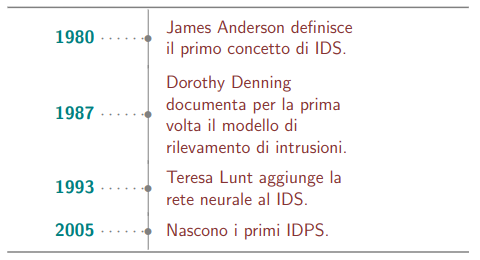
\includegraphics[width=0.45\textwidth]{image/IDStimeline.png}
\end{wraptable} 
Un IDS (Intrusion Detection System), così definito dal NIST, è un processo di monitoraggio degli eventi che si verificano in un computer o in una rete e dell'analisi di essi per individuare segni di intrusioni, quest'ultime vengono definite come tutti i tentativi di compromettere la confidenzialità, l'integrità, la disponibilità o di aggirare meccanismi di sicurezza di un computer o di una rete\cite{nistIDS}.\\
La prima elaborazione del concetto di sistema di IDS risale al 1980 e si deve in particolare a James Anderson, analista presso la National Security Agency. Il sistema di Anderson comprendeva un insieme di strumenti per amministratori di sistema per poter esaminare i registri di audit\cite{ComputerSecurityThreat}. Nel febbraio del 1987, Dorothy E. Denning, assistita da Peter G. Neumann presso IDS International, pubblicò un documento intitolato "An Intrusion Detection Model", nel quale introdussero miglioramenti al modello di Anderson\cite{AnIntrusionDetectionModel}. Il modello di Denning consisteva in un sistema esperto basato su regole per rilevare pattern di intrusioni note e una componente di rilevazione statistica basata su profili di utenti, sistemi host e sistemi di destinazione, diventando noto come Intrusion Detection Expert System. Nel 1990, Teresa F. Lunt, autrice di "IDES: An Intelligent System for Detecting Intruders", aggiunse l'ultimo componente al modello di Denning: una rete neurale artificiale capace di adattarsi agli eventi e modificarsi\cite{IDES}.\\
Un sistema di rilevamento delle intrusioni (IDS) è un dispositivo software o un'applicativo che monitora una rete o i dispositivi su cui è installato. Quando rileva un'anomalia, la segnala a un sistema di raccolta di eventi di sicurezza (SIEM), che utilizza tecniche di filtraggio degli allarmi per distinguere falsi positivi da attività dannose\cite{taxonomy}.\\
Gli IDS, come i firewall, vengono utilizzati per bloccare intrusioni nella rete, ma differiscono dalla risposta a tali intrusioni. I sistemi di rilevamento delle intrusioni possono anche avere scopi specifici se integrati con strumenti personalizzati, come l'utilizzo di un honeypot per attirare e caratterizzare il traffico dannoso\cite{idsFirewall}.\\
Recentemente, sono stati realizzati prodotti denominati sistemi di rilevamento e prevenzione delle intrusioni (IDPS), i quali possiedono la capacità di rispondere proattivamente alle intrusioni rilevate. Gli IDPS hanno, inoltre, la capacità di fermare un attacco rilevato, registrare gli eventi, avvisare gli amministratori, bloccare la minaccia e generare rapporti. A differenza degli IDS, gli IDPS devono essere posizionati "in linea", monitorando in tempo reale per bloccare intrusioni, inviare allarmi, rifiutare pacchetti dannosi e correggere errori di rete\cite{idps}.\\


\subsection{Tipologie di IDS}
Secondo il NIST è possibile classificare gli IDS in base alla loro posizione o all'approccio di rilevamento, in base alla posizione si dividono in:
\begin{itemize}
	\item \textbf{NIDS (Network IDS)}: posizionati strategicamente nella rete, monitorano il traffico da e verso tutti i dispositivi, analizzando idealmente sia l'entrata che l'uscita. L'uso di reti neurali artificiali può migliorare i tassi di rilevamento grazie alla capacità di analizzare grandi volumi di dati in modo intelligente e apprendere dagli errori, sviluppando un sistema di avviso precoce\cite{taxonomy}.
	\item \textbf{HIDS (Host IDS)}: operano su singoli host o dispositivi, monitorando solo i pacchetti in entrata e in uscita. Consentono l'analisi del traffico di rete criptato, una volta arrivato all'host\cite{taxonomy}.
\end{itemize}
In base all'approccio di rilevamento invece si dividono in:
\begin{itemize}
	\item \textbf{Signature-based}: ricerca pattern specifici, simile all'azione degli antivirus per individuare sequenze di byte o istruzioni malevole conosciute. Risponde velocemente ad attacchi noti, ma può non riconoscere nuovi attacchi senza pattern noti\cite{signature}.
	\item \textbf{Anomaly-based}: utilizza l'apprendimento automatico per creare un modello di attività affidabile e confrontare il nuovo comportamento. Riesce a rilevare attacchi sconosciuti, ma potrebbe generare falsi positivi, identificando attività legittime come malevoli\cite{anomaly}.
\end{itemize}

\subsection{Darktrace: panoramica}
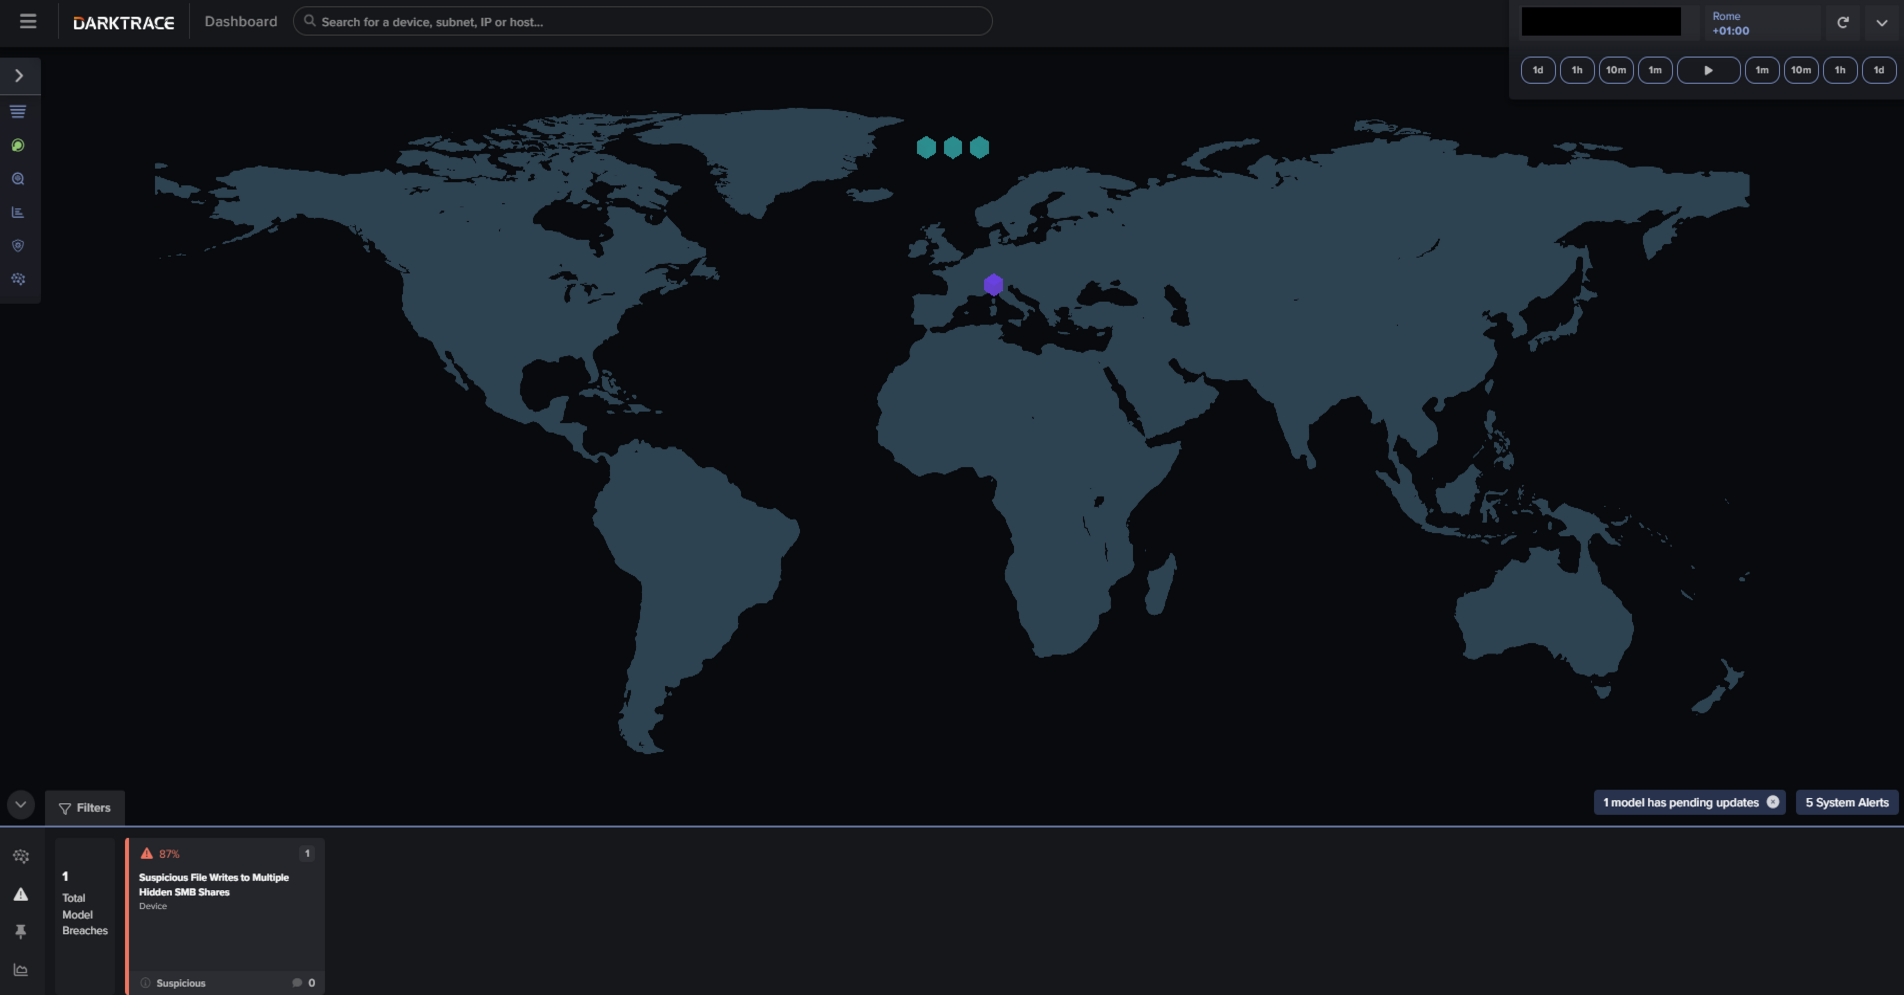
\includegraphics[width=\textwidth]{image/darktrace.png}
Darktrace, fondata nel 2013 a Cambridge, Regno Unito, da ex-dipendenti dell'intelligence governativa e matematici dell'Università di Cambridge, è un Intrusion Detection and Prevention System (IDPS) che immagazzina e analizza il traffico di rete per lunghi periodi al fine di identificare correlazioni e modelli comportamentali.\\
Utilizzando avanzate tecniche di probabilità bayesiana e machine learning, Darktrace crea un profilo comportamentale unico per ciascun utente e dispositivo all'interno dell'ambiente di rete. Inoltre, è in grado di raggruppare gli utenti e i dispositivi in base ai loro comportamenti, consentendo così di rilevare anomalie nel caso in cui un utente o un dispositivo si discosti dal comportamento tipico del suo gruppo.\\
Operando in tempo reale e analizzando il traffico di rete in modo continuo, Darktrace è in grado di identificare anche gli attacchi "zero-day", che non seguono schemi precedentemente noti. Per garantire l'affidabilità delle segnalazioni, Darktrace utilizza un'intelligente soglia di rilevamento che contestualizza e aggiorna costantemente le segnalazioni in base alle rilevazioni precedenti, riducendo al minimo i falsi positivi e mitigando il rischio di distorsioni dovute al tasso di base.\\
Darktrace è composto da quattro moduli distinti: Darktrace PREVENT, Darktrace DETECT, Darktrace RESPOND e Darktrace HEAL. Tuttavia, durante il tirocinio, ci concentreremo esclusivamente sui moduli DETECT e RESPOND, in quanto sono gli unici utilizzati durante l'esperienza pratica\cite{threat1}.


\subsection{Darktrace DETECT}
Darktrace DETECT offre un'interfaccia che segnala le anomalie e fornisce gli strumenti per valutare se sono comportamenti legittimi nell'ambiente lavorativo o malevoli. Le violazioni dei modelli possono essere parte di un incidente dell'AI Analyst o un'allerta autonoma, comunicando agli utenti tramite l'interfaccia Threat Visualizer comportamenti anomali di dispositivi o account\cite{threat2}.\\
Un modello è composto da tre elementi fondamentali:
\begin{itemize}
	\item Condizioni del modello: sono componenti che, quando soddisfatte, provocano una violazione del modello. Ogni componente è composto da una metrica con le proprie condizioni filtro, come l'utilizzo di protocolli specifici o pacchetti HTTP con User Agent rari. Questi elementi, insieme, costituiscono la logica del modello.
	\item Modulazione del punteggio: comprende quattro modelli che influenzano il comportamento del modello quando viene attivato. Il modello standard specifica che una continua violazione nel tempo diminuisce il punteggio, ma esistono anche altre modalità: una modulazione che mantiene lo stesso punteggio nel tempo e un'altra che aumenta il punteggio dopo le prime violazioni e poi lo diminuisce.
	\item Azioni del modello: sono azioni di sistema che possono essere attivate in risposta a una violazione del modello. Queste azioni possono includere l'invio di email o notifiche HTTP. Inoltre, è possibile selezionare una criticità diversa da quella standard o segnalare la violazione come "Informational"\cite{model}.
\end{itemize}
Solo una parte degli incidenti viene segnalata dall'\textit{AI Analyst} di Darktrace, il quale raccoglie molteplici informazioni rilevanti e le presenta in un formato facilmente comprensibile per l'operatore. Questo strumento investiga, analizza e categorizza le minacce all'interno dell'ambiente, identificando incidenti potenzialmente interessanti e insoliti, spesso raggruppandoli per un singolo dispositivo. Gli incidenti che coinvolgono più dispositivi sono classificati come incidenti "\textit{cross-network}". L'\textit{AI Analyst} non si limita a investigazioni autonome e non sollecitate, ma è anche disponibile su richiesta per un dispositivo selezionato da parte dell'operatore.\\
Per quanto riguarda le allerte autonome, è compito dell'analista indagare su di esse utilizzando gli strumenti forniti da Darktrace DETECT per rispondere alle 5 W:
\begin{enumerate}
	\item Who?: identificare chi ha scatenato l'allarme.
	\item What?: comprendere quale azione è stata compiuta.
	\item When?: determinare quando sono avvenute tali operazioni.
	\item Where?: individuare il dispositivo o il luogo in cui sono state effettuate tali operazioni.
	\item Why?: capire il motivo per cui Darktrace ha segnalato questa anomalia.
\end{enumerate}
Se la legittimità dell'attività non è immediatamente chiara attraverso le informazioni fornite dalla violazione del modello, è consigliabile contattare l'utente finale, poiché la consultazione e la collaborazione con gli utenti sono fondamentali per una valutazione completa della situazione\cite{threat2}.

\subsection{Darktrace RESPOND}
Darktrace RESPOND/Network è progettato per gestire minacce di sicurezza di alto livello, come ad esempio i ransomware. Utilizzando due approcci distinti, può interrompere le connessioni malevole sia attraverso il reset TCP che integrandosi direttamente con il firewall esistente, inviando messaggi direttamente a esso.\\
Il flag RST del protocollo TCP è una componente delle comunicazioni standard tra dispositivi: quando un endpoint riceve un pacchetto con questo flag attivato, la connessione viene immediatamente interrotta. Darktrace rileva attività sospette e, in caso di anomalie, invia pacchetti di reset TCP a entrambi i dispositivi coinvolti, sia all'interno che all'esterno della rete, per interrompere la connessione malevola. Gli indirizzi IP dei pacchetti di reset sono falsificati per far credere ai dispositivi che non provengano da Darktrace, ma l'uno dall'altro.\\
Darktrace RESPOND può attuare una serie di azioni proattive, misurate e automatizzate in risposta a minacce informatiche confermate rilevate in tempo reale. I componenti di Darktrace RESPOND possono essere utilizzati in due modalità distinte:
\begin{itemize}
	\item \textbf{Modalità di conferma umana}: le azioni di Darktrace RESPOND rimarranno in 
	sospeso fino a quando un operatore umano non conferma o ignora 
	la segnalazione del modulo RESPOND.
	\item \textbf{Modalità autonoma o parzialmente autonoma}: in modalità completamente 
	autonoma, RESPOND risponde automaticamente alle minacce, mentre nella modalità 
	parzialmente autonoma, può essere attivato autonomamente al di fuori degli orari 
	lavorativi, ma richiede conferma umana per il resto del tempo.
\end{itemize}
Darktrace RESPOND reagisce alle violazioni dei modelli offrendo l'opzione di impostare 
un inibitore, che è un'azione finalizzata a contrastare il comportamento anomalo del 
dispositivo o dell'utente. Gli inibitori disponibili includono:
\begin{itemize}
	\item \textbf{Bloccare le connessioni corrispondenti}: interrompe le connessioni dal dispositivo all'endpoint di destinazione identificato nell'incidente, sulla porta di destinazione osservata.
	\item \textbf{Imporre il pattern di vita}: consente al dispositivo di effettuare solo connessioni e trasferimenti di dati considerati normali da Darktrace, basati sui modelli di vita definiti per quel dispositivo. Qualsiasi attività che si discosti da questi modelli viene bloccata.
	\item \textbf{Imporre il pattern di vita del gruppo}: permette al dispositivo di intraprendere le stesse connessioni e trasferimenti di dati che sono comuni tra i dispositivi nel suo gruppo di pari, basandosi sui modelli di vita del gruppo.
	\item \textbf{Quarantena del dispositivo}: blocca tutto il traffico di rete in entrata e in uscita dal dispositivo, isolandolo dalla rete.
	\item \textbf{Blocco di tutti i traffici in uscita}.
	\item \textbf{Blocco di tutti i traffici in entrata}\cite{respond}.
\end{itemize}
	
	\chapter{Sperimentazione con Tpot e Darktrace}
\begin{enumerate}
	\item Implementazione di Tpot e analisi dei risultati
	\begin{enumerate}
		\item Configurazione di base
		\item Script e automazioni
		\item Dati raccolti
	\end{enumerate}
	\item Monitoraggio delle reti con Darktrace
	\begin{enumerate}
		\item Definizione e origine degli IDS
		\item Minacce importanti rilevate
		\item Esempi di segnalazioni quotidiane
	\end{enumerate}
	\item Integrare Darktrace e Tpot per una maggiore sicurezza
\end{enumerate}
\section{Implementazione di Tpot e analisi dei risultati}
\subsection{Configurazione di base}
Per prima cosa, è fondamentale verificare di avere tutti i prerequisiti necessari per l'installazione corretta dell'honeypot, questi prerequisiti sono: un indirizzo IP fornito da un server DHCP e una connessione ad Internet, spazio di archiviazione minimo necessario, spazio di memoria RAM. Queste ultime due possono variare in base alla tipologia di installazione \textit{standalone} o \textit{distribuita}. Successivamente, dalla pagina ufficiale Github di T-Pot deve essere scaricata l'immagine ISO; si tratta di un file che contiene l'immagine del sistema operativo preconfigurato con tutti gli strumenti e le funzioni necessarie per T-Pot. Una volta scaricata l'immagine ISO, il passo successivo è l'installazione effettiva dell'immagine. Ciò deve avvenire seguendo attentamente i passaggi indicati fino al completamento dell'installazione, potendo scegliere quale dei tre tipi installare:
\begin{itemize}
	\item \textit{Standalone}: è la versione completa in cui vengono installati tutti i sistemi per far si che funzioni autonomamente.
	\item \textit{Sensor}: è la versione che installa solo il sensore, quindi comprende solo gli honeypot e non i pacchetti per la gestione via interfaccia web.
	\item \textit{Hive}: versione che non include honeypot ma solo programmi per il collegamento ed il controllo da remoto in quanto adibita a raccogliere i dati dalle versioni \textit{sensor}, grazie all'uso di tunnel SSH.
\end{itemize}
Una volta completata l'installazione, viene visualizzato un prompt contenente le informazioni per connettersi al sistema da remoto, questo può essere effettuato tramite l'interfaccia web contenente un terminale oppure tramite connessione SSH. La seguente immagine viene visualizzata in caso T-Pot sia stato installato correttamente ed è pronto all'uso.\\
\begin{center}
	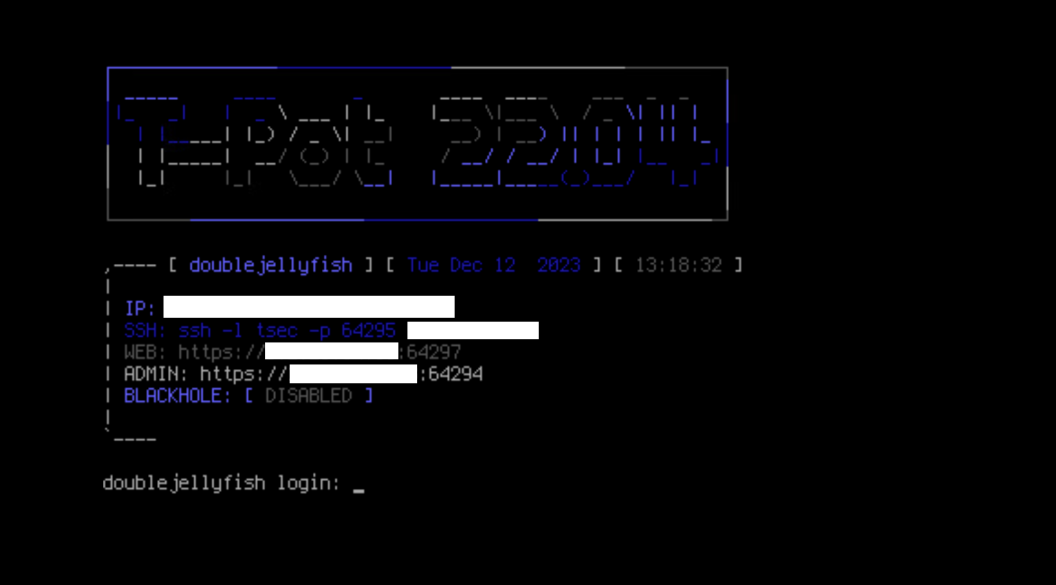
\includegraphics[width=0.8\textwidth]{image/fineInstallazione.png}
\end{center}
Dopo aver completato l'installazione di T-Pot, è necessario apportare alcune modifiche e configurazioni aggiuntive per assicurarsi che funzioni correttamente.\\
Il primo passaggio dopo l'installazione è modificare il file \textit{/etc/network/interface} per configurare correttamente l'interfaccia di rete primaria dell'honeypot. Dopo aver apportato le modifiche al file di configurazione, è necessario riavviare l'interfaccia di rete affinché le modifiche abbiano effetto. Successivamente, è importante installare e configurare il server di posta Postfix utilizzando il gestore di pacchetti apt. Postfix è necessario per consentire a T-Pot di inviare mail contenenti le segnalazioni di connessioni malevole. \\
Durante la configurazione di Postfix, è essenziale assicurarsi che sia configurato per utilizzare la porta 587 per le comunicazioni email anziché la porta standard 25. Ciò è particolarmente importante perché la porta 25 viene occupata dagli Mailoney, mentre la porta 587 offre una maggiore sicurezza.

\subsection{Script e automazioni}
Lo scopo del progetto era di inviare dati degli attacchi subiti da T-Pot al SIEM tramite plugin o programmi esistenti, ma poiché non erano disponibili soluzioni adatte alle esigenze aziendali, è stato sviluppato uno script per analizzare i log dei principali honeypot: 
\begin{itemize}
	\item Dionaea: utilizzato per monitorare la porta legata al protocollo FTP(21).
	\item Cowrie: utilizzato per monitorare le porte legate ai protocolli SSH e Telnet(22, 23).
	\item Tanner: utilizzato per monitorare le porte legate al protocollo HTTP(80, 8080).
	\item Citrixhoneypot: utilizzato per monitorare le porte legate al protocollo HTTPS(443).
	\item Honeytrap: utilizzato per monitorare un gruppo di porte non standard, le porte maggiori di 1024.
\end{itemize}
Lo script estrae le informazioni rilevanti dai log di ogni honeypot e le formatta per l'integrazione con il SIEM.\\
\begin{lstlisting}[language=bash,caption={CEF\_Script.sh}]
#!/bin/bash

honeytrapFile="/data/honeytrap/log/attacker.log"

honeytrapBackup="/home/tsec/script/backup/honeytrap/backup.log"

messaggio=""

if [ ! -e "$honeytrapBackup" ]; then
touch $honeytrapBackup
fi

diffHoneytrap=$(diff $honeytrapFile $honeytrapBackup)
if [ "$diffHoneytrap" != "" ]; then
tmpHoneytrap="/tmp/diffHoneytrap"
diff $honeytrapFile $honeytrapBackup | grep -E '^<|^>' | sed 's/^< //' > $tmpHoneytrap
cp $honeytrapFile $honeytrapBackup
chown tsec:tsec $honeytrapBackup
honeytrapAttaccoPort=$(awk -F'[: ]+' '/^.*tcp/ { print "DeviceName=Honeypot DestinationIP="$11" DestinationPort="$12" ApplicationProtocol= SourceIP="$8" SourcePort="$9"" }' $tmpHoneytrap | sort -u)
if [ ! -z "$honeytrapAttaccoPort" ]; then
messaggio+="Sono state riscontrate le seguenti connessioni alle porte dell'honeypot:\n$honeytrapAttaccoPort\n"
messaggioCEF=$(awk -F'[: ]+' '/^.*tcp/ { print $12" "$8 }' $tmpHoneytrap | sort | uniq -c | awk '{print "reason=Honeytrap cn1="$1" src="$3" dpt="$2}')

echo "$messaggioCEF" | while IFS= read -r linea; do
if [ ! -z "$linea" ]; then
logger -p local4.warn -P 514 -n 127.0.0.1 --rfc3164 -t CEF "0|Honeypot-Test|Honeypot-Test|0.1|event-honeypot-test|end|TRAFFIC|$linea"
fi
done
fi
rm -f $tmpHoneytrap
fi

if [ ! -z "$messaggio" ]; then
echo -e "To: provaAlertEmailMatteo@gmail.com\nSubject: Connessioni all'honeypot\n$messaggio" >> /tmp/mailTemp.txt
/usr/sbin/sendmail provaAlertEmailMatteo@gmail.com < /tmp/mailTemp.txt
rm -f /tmp/mailTemp.txt
fi
\end{lstlisting}
Ecco una spiegazione delle principali azioni svolte dallo script:
\begin{enumerate}
	\item Viene definito il percorso del file di log dell'honeypot e il percorso del file di backup che conterrà una copia del file di log per confronti successivi.
	\item Se il file di backup non esiste, viene creato.
	\item Viene eseguito un confronto tra il file di log attuale e quello di backup per individuare eventuali differenze.
	\item Se vengono rilevate delle differenze, vengono estratte le informazioni sulle connessioni di attacco dal file di log attuale.
	\item Queste informazioni vengono aggiunte a un messaggio di notifica che sarà inviato tramite email.
	\item Viene generato un messaggio nel formato CEF (Common Event Format) per ciascuna connessione di attacco trovata.
	\item Infine, se è stato creato un messaggio di notifica, viene creato un file temporaneo contenente il testo dell'email di notifica e viene inviata l'email utilizzando il comando sendmail.
\end{enumerate}
Questo processo viene effettuato per i cinque honeypot elencati precedentemente. Per far sì che lo script esegua il controllo dei log ogni minuto, è necessario configurare il file crontab. Questo file è collegato al comando crontab, il quale, all'avvio del sistema, esegue un demone che legge il file ogni minuto.\\
Successivamente, è necessario creare un altro script che permetta la cancellazione delle cartelle di backup utilizzate per il confronto all'avvio del sistema, al fine di mantenere la logica del programma integra.

\clearpage

\begin{lstlisting}[language=bash,caption={Delete\_Script.sh}]
#!/bin/bash

# Specifica i percorsi dei file che vuoi cancellare
dionaeaBackup="/home/tsec/script/backup/dionaea/backup.json"
cowrieBackup="/home/tsec/script/backup/cowrie/backup.json"
tannerBackup="/home/tsec/script/backup/tanner/backup.json"
citrixhoneypotBackup="/home/tsec/script/backup/citrixhoneypot/backup.log"
honeytrapBackup="/home/tsec/script/backup/honeytrap/backup.log"

# Cancella i file
rm -f $dionaeaBackup $cowrieBackup $tannerBackup
rm -f $citrixhoneypotBackup $honeytrapBackup

# Aggiungi altre operazioni di pulizia, se necessario
echo "File cancellati con successo."
\end{lstlisting}
Una volta creato quest'ultimo script, è necessario creare un servizio che esegua quest'ultimo script ad ogni avvio della macchina. Questo può essere fatto utilizzando i servizi di systemctl con il seguente codice:
\begin{lstlisting}[caption={Delete\_Backup.service}]
	[Unit]
	Description=Script per cancellare file prima del riavvio
	
	[Service]
	Type=oneshot
	ExecStart=/usr/local/bin/delete_backup.sh
	
	[Install]
	WantedBy=multi-user.target
\end{lstlisting}

\subsection{Dati raccolti}
I dati qui mostrati riguardano tutti gli attacchi subiti dall'honeypot, non solo quelli raccolti dallo script, nell'arco temporale di una settimana in cui T-Pot è stato esposto a Internet.\\
\begin{tikzpicture}
	\begin{axis}[ybar,
		bar width=1,
		ymin=0,
		enlarge x limits={abs=1},
		xtick=data,
		point meta=y*100,
		nodes near coords={\pgfmathprintnumber\pgfplotspointmeta\%},
		nodes near coords style={/pgf/number format/precision=3,
			/pgf/number format/fixed},
		xticklabels={TCP,UDP,ICMP},
		yticklabel={\pgfmathparse{\tick*100}\pgfmathprintnumber{\pgfmathresult}\%},
		tickwidth=0,
		]
		
		\addplot table[x expr=\coordindex,y index=0,row sep=\\] {0.913\\0.047\\0.038\\};
	\end{axis}
\end{tikzpicture}\\
L'analisi dei dati raccolti rivela che la quasi totalità dei pacchetti ricevuti è di tipo TCP, rappresentando il 91,3\% del totale, seguito da UDP con il 4,7\% e ICMP con il 3,8\%. Questo è in linea con il fatto che il protocollo TCP richiede un maggior numero di pacchetti per la sua affidabilità.\\
\begin{tikzpicture}
	\begin{axis}[ybar,
		bar width=1,
		ymin=0,
		enlarge x limits={abs=1},
		xtick=data,
		point meta=y*100,
		nodes near coords={\pgfmathprintnumber\pgfplotspointmeta\%},
		nodes near coords style={/pgf/number format/precision=2,
			/pgf/number format/fixed},
		xticklabels={US,RU,CN,UK,NL,VT,IN,SG,DE,WD},
		yticklabel={\pgfmathparse{\tick*100}\pgfmathprintnumber{\pgfmathresult}\%},
		tickwidth=0,
		]
		
		\addplot table[x expr=\coordindex,y index=0,row sep=\\] {0.316\\0.206\\0.076\\0.064\\0.059\\0.056\\0.054\\0.050\\0.048\\0.068\\};
	\end{axis}
\end{tikzpicture}\\
Mentre dal punto di vista geografico, gli Stati Uniti d'America, la Russia e la Repubblica Popolare Cinese sono i principali attori; infatti, contribuiscono complessivamente al 59,8\% di tutti gli attacchi registrati, seguiti da altri paesi come Regno Uniti, Paesi Bassi, Vietnam, India, Singapore, Germania e il resto del mondo, che rappresenta il 6,8\%.\\
\begin{tikzpicture}
	\begin{axis}[ybar,
		bar width=1,
		ymin=0,
		enlarge x limits={abs=1},
		xtick=data,
		point meta=y*100,
		nodes near coords={\pgfmathprintnumber\pgfplotspointmeta\%},
		nodes near coords style={/pgf/number format/precision=3,
			/pgf/number format/fixed},
		xticklabels={0,21,22,23,25,80,102,443,>1024},
		yticklabel={\pgfmathparse{\tick*100}\pgfmathprintnumber{\pgfmathresult}\%},
		tickwidth=0,
		]
		
		\addplot table[x expr=\coordindex,y index=0,row sep=\\] {0.010\\0.014\\0.448\\0.053\\0.037\\0.103\\0.011\\0.148\\0.176\\};
	\end{axis}
\end{tikzpicture}\\
Nel dettaglio delle porte più attaccate, la porta 22 (SSH) risulta essere quella bersagliata più frequentemente, il 44,8\% di tutti gli attacchi diretti sono a questa porta. Le porte 443 (HTTPS) e 80 (HTTP) seguono rispettivamente con il 14,8\% e il 10,3\%. Altre porte di rilevanza includono la porta 23 (Telnet) e la porta 25 (SMTP), mentre le porte non standard, quelle non standard ($>$1024), contribuiscono in misura minore agli attacchi subiti.

\section{Monitoraggio delle reti con Darktrace}
\subsection{Minacce importanti rilevate}
Nel contesto di questa sezione, saranno esaminati tre casi di anomalie rilevate e risolte utilizzando Darktrace.\\
Il primo caso riguarda il worm Conficker (CVE-2008-4250), scoperto nel 2008, che sfrutta una vulnerabilità non ancora corretta di Microsoft Windows, al fine di violare la password di amministratore locale. Una volta ottenuto il controllo di un dispositivo, il worm cerca di diffondersi ad altre macchine nella rete. Darktrace ha riconosciuto questa minaccia tramite il rilevamento di grandi richieste DNS domini generati da algoritmi (DGA). Di fronte a tale minaccia, Darktrace ha messo automaticamente il dispositivo interessato in quarantena, rimuovendolo dalla rete fino a quando un operatore umano non ha deciso di rilasciarlo.\\
La seconda anomalia significativa coinvolge l'uso di strumenti di attacco e ricognizione, come Nmap, Nessus o OpenVAS, da parte di un dispositivo di rete per condurre scansioni e catalogare informazioni su indirizzi IP, porte aperte, sistemi operativi e vulnerabilità. Darktrace ha riconosciuto quante e quali porte/servizi sono stati scansionati ed è intervenuto bloccando tutte le connessioni in uscita del dispositivo coinvolto. L'analista responsabile ha poi contattato il cliente per informarlo sull'attività sospetta all'interno della sua rete.\\
Infine, nel terzo caso, Darktrace ha rilevato un'anomalia denominata "Ransomware / SMB Reads then Writes with Additional Extensions". In questo scenario, è stato osservato un dispositivo che ha letto un gran numero di file SMB con un'estensione specifica, seguito dalla scrittura di un numero corrispondente di file con un'estensione aggiuntiva. Questo comportamento poteva essere indicativo di un attacco ransomware. Darktrace ha consigliato di esaminare attentamente i file scritti per verificare se corrispondessero a un'estensione tipica dei ransomware.

\subsection{Esempi di segnalazioni quotidiane}
Le segnalazioni quotidiane possono essere suddivise in due categorie: comune e media gravità. Tra gli incidenti comuni segnalati quotidianamente troviamo:
\begin{itemize}
	\item \texttt{Plaintext password}: questo tipo di segnalazione indica l'individuazione di login inviati in chiaro, ovvero senza alcuna cifratura delle credenziali. Questi eventi possono verificarsi nei protocolli HTTP o LDAP. I login scoperti vengono successivamente inclusi nel report settimanale inviato all'azienda.
	\item \texttt{Possible Unencrypted Password File On Server}: questo incidente si verifica quando un dispositivo apre un documento con nel titolo le parole "password", "pwd" o "secret", e non utilizza un formato noto per la sicurezza, ma un formato comune come .doc o .xlsx. Tali file vengono segnalati nel report settimanale.
	\item \texttt{Anonymous NTLM logins}: questa segnalazione avviene quando un dispositivo tenta di autenticarsi con altri dispositivi tramite NTLM utilizzando un account utente anonimo. Questi tentativi di login anonimi vengono poi inclusi nel report settimanale consegnato al cliente.
\end{itemize}
Le segnalazioni di media gravità, che richiedono un'analisi più approfondita, includono:
\begin{itemize}
	\item \texttt{Suspicious Domain}: questo tipo di segnalazione avviene quando un dispositivo si connette a un dominio esterno raro, non comunemente visitato all'interno della rete, con un dominio di primo livello (TLD) associato ad attività dannose, come ad esempio "example.top". Il compito dell'analista è verificare la legittimità del sito, utilizzando strumenti come Cisco Talos o VirusTotal.
	\item \texttt{Unusual Admin RDP Session}: questa segnalazione si verifica quando viene effettuata una connessione RDP (Remote Desktop Protocol) con credenziali di amministratore. L'analista contatta solitamente il cliente per verificare la legittimità dell'operazione.
	\item \texttt{BitTorrent}: viene segnalato quando un dispositivo stabilisce connessioni peer-to-peer BitTorrent, spesso associato alla condivisione di dati protetti da copyright o ad altre informazioni indesiderate. In questo caso, si consiglia al cliente di indagare sulla quantità di dati scaricati e di disinstallare il programma dai dispositivi aziendali.
\end{itemize}

\section{Integrare Darktrace e Tpot per una maggiore sicurezza}
L'integrazione di Darktrace e T-Pot offre una serie di vantaggi significativi per la sicurezza informatica. Da un lato, Darktrace con la sua capacità di rilevare e prevenire intrusioni in tempo reale, consente di identificare e rispondere prontamente alle minacce attive. Tuttavia, può essere limitato dalla sua capacità di rilevare solo le minacce già note o le firme di attacco conosciute. D'altro, T-Pot agisce come esca per attirare gli attaccanti e raccogliere informazioni sulle loro tattiche e strategie. Integrando questi due strumenti, è possibile prevenire gli attacchi esterni, i quali vengono attratti e intrappolati da T-Pot; contemporaneamente è possibile bloccare gli attacchi che si verificano all'interno della rete, migliorando così complessivamente la sicurezza dell'ambiente informatico.
	
	\chapter{Conclusioni}
Il lavoro illustrato in questa tesi ha segnato un importante traguardo nell'ambito della sicurezza informatica aziendale, attraverso l'efficace implementazione di un honeypot e la gestione di un IDPS. L'adozione di un progetto open-source predefinito ha agevolato il percorso, permettendo di dedicare maggiori risorse all'espansione e al potenziamento dei servizi offerti. Sebbene ciò abbia semplificato la fase iniziale di installazione, l'integrazione con il SIEM ha richiesto un impegno sia di tempo che di studio aggiuntivo, evidenziando l'importanza di una profonda comprensione del contesto aziendale e dei suoi requisiti specifici.\\
Il percorso seguito, partendo dalla fase preliminare di studio e definizione degli obiettivi, attraverso la fase di progettazione e l'effettiva implementazione del progetto, ha dimostrato di essere un metodo efficace nel conseguimento degli obiettivi prefissati. L'honeypot sviluppato è risultato efficace nel mitigare il traffico dannoso proveniente dagli attaccanti, mentre le competenze acquisite nell'utilizzo di Darktrace hanno notevolmente arricchito le capacità difensive aziendali.\\
Per quanto riguarda i futuri sviluppi, il prossimo passo potrebbe essere quello di valutare l'offerta del servizio ai clienti, qualora vengano riscontrati benefici a lungo termine, da affiancare al monitoraggio già fornito dal SOC tramite Darktrace. In tal senso, potrebbe essere considerata l'installazione delle distribuzioni sensore di T-pot all'interno delle subnet utilizzate dai clienti. Queste distribuzioni sarebbero in grado di rilevare e bloccare qualsiasi attività sospetta tramite il SIEM, offrendo così un livello aggiuntivo di protezione.\\
Al fine di agevolare l'adozione di questa soluzione da parte dei clienti, è stata redatta una documentazione esaustiva, finalizzata a semplificare l'implementazione e l'utilizzo della piattaforma, garantendo che i vantaggi e le potenzialità dell'honeypot e dell'IDPS possano essere pienamente sfruttati. La ricerca continua di miglioramenti e l'adattamento alle esigenze emergenti del panorama della sicurezza informatica rimarranno al centro delle future attività, con l'obiettivo primario di garantire una protezione sempre più efficace contro le minacce in continua evoluzione.
	
	\chapter{Bibliografia}
	\printbibliography[heading=none]
	
	\chapter{Ringraziamenti}
	
\end{document}
